\section{Exercise 1: BPEL processes}

\subsection{parallelization}

In order to parallelize the operations inside the BPEL process, the
\hl{bpel:flow} tag was used. Sequences (\hl{bpel:sequence}) placed inside are
executed in parallel.\\

Before describing which activities were parallelized and why, here's a short
list describing each activity.

\begin{enumerate}
    \item \textbf{receiveInput} - Retrieves the request.
    \item \textbf{PrepareResponse} - Creates an empty response tree.
    \item \textbf{AssignSearchRequest (1)} - Creates a request with the given
        parameters. The created request will be sent to the SoftLibrary web
        service.
    \item \textbf{InvokeSearchBooks (1)} - Sends the request to the SoftLibrary web
        service and stores the result in a variable.
    \item \textbf{AssignSearchRequest (2)} - Creates a request for the
        NationalLibrary web service.
    \item \textbf{InvokeSearchBooks (2)} - Sends the request to the NationalLibrary
        web service and stores the result in a variable.
    \item \textbf{AssignResultSoftLib} - Performs an xsl transformation to
        adapt the response from both web service, and stores the result
        in the previously created empty response.
    \item \textbf{replyOutput} - Sends the response.
\end{enumerate}
\

Below are the dependencies between the operations, and which operations were
parallelized considering these dependencies.\\

\begin{figure}[h!]
    \centering
    \begin{subfigure}[b]{0.16\textwidth}
        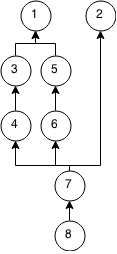
\includegraphics[width=\textwidth]{images/deps.png}
        \caption{dependencies}
    \end{subfigure}%
    ~
    \begin{subfigure}[b]{0.16\textwidth}
        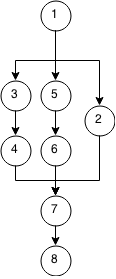
\includegraphics[width=\textwidth]{images/parallel.png}
        \caption{parallelization}
    \end{subfigure}
\end{figure}

\begin{lstlisting}[language=XML]
<bpel:sequence name="main">
    <bpel:receive name="receiveInput" ... />

	<bpel:flow>
        <bpel:sequence>
    		<bpel:assign name="PrepareResponse" ...>...</bpel:assign>
        </bpel:sequence>
        
        <bpel:sequence>
    		<bpel:assign name="AssignSearchRequest" ...>...</bpel:assign>

    		<bpel:invoke name="InvokeSearchBooks" .../>
        </bpel:sequence>
		
        <bpel:sequence>
    		<bpel:assign name="AssignSearchRequest" ...>...</bpel:assign>

    		<bpel:invoke name="InvokeSearchForBooks" .../>
        </bpel:sequence>
    </bpel:flow>
				
	<bpel:assign name="AssignResultSoftLib" ...>...</bpel:assign>
    
    <bpel:reply name="replyOutput" .../>
</bpel:sequence>
\end{lstlisting}

\subsection{XSLT}

The responses given by both web services are different (different tags and data
types). Our final objective will be to instantiate Book objects
(\hl{softarch.portal.data.Book}) from our \emph{web\_portal}. In order to do
that, at one point in the process we will need to do some modification to the
responses. We could retrieve both responses in intermediate Book classes (one
for each web service), and then convert them into the intended Book class. Or we
can let the bpel process delegate this task to \emph{XSLT}.\\

\emph{XSLT} is a language using XML to transform XML documents in other formats.
In our case, we want to transform both XML responses into an unified XML
response. The books will need to conform to a common "interface", the Book
comlexType defined in \hl{LibrarySearchArtifacts.wsdl}. The XSLT transform
is called by the \textbf{AssignResultSoftLib} activity and handled by the
\hl{books.xsl} file which can be seen below.\\

\lstinputlisting[language=XML]{../LibrarySearch/books.xsl}
\

Once these modifications are made, we need to do the following modification in
\hl{LibrarySearchArtifacts.wsdl} (comment a line, uncomment another one). The
uncommented lines tells that a BookList is composes of \hl{tns:Book} elements,
which is the type to which our unified response conforms to.\\

\begin{lstlisting}
<complexType name="BookList">
	<sequence>
		<!--<xsd:any minOccurs="0" maxOccurs="unbounded" processContents="skip"></xsd:any>-->
		<element name="book" type="tns:Book" maxOccurs="unbounded" minOccurs="0"></element>
	</sequence>
</complexType>
\end{lstlisting}
\

\begin{framewarning}
    Using XSLT might not be the best course of action. It is written in XML, so
    it's far from being pleasant to read. It is also far from being simple or
    easy to debug, and writing a working xsl file may take some time. The
    alternative, doing the unification job in the \emph{web\_portal} in Java,
    would have been much simpler, even if it would have meant cluttering the
    portal code.
\end{framewarning}

\newpage
